
Outline:

- Motivace
\section{Úvod}

\begin{frame}
  \frametitle{Motivace}
  \begin{itemize}
    \item xx
  \end{itemize}
\end{frame}
\begin{frame}
  \frametitle{Stránka s ovládacími prvky a reklamami}
  \begin{center}
    
\includegraphics[height=.9\textheight]{img/root-balast.png}
  \end{center}
\end{frame}

\begin{frame}
  \frametitle{Stránka v zobrazení čtečky}
  \begin{center}
    \includegraphics[height=.9\textheight]{img/root-čtečka.png}
  \end{center}
\end{frame}

\section{Jak zkonvertujeme HTML do PDF pro čtečku?}

\begin{frame}
  \frametitle{Reader mode pro skripty}
  \begin{tabular}{ll}
    Readability.js & \url{https://github.com/mozilla/readability}\\
    Python-readability & \url{https://github.com/buriy/python-readability}\\
    Rdrview: &\url{https://github.com/eafer/rdrview}\\
  \end{tabular}

\end{frame}

\section{Responzivní design v \LaTeX u}

\begin{frame}
  \frametitle{Balíček \texttt{responsive}}

  Experimentální balíček inspirovaný metodami responzivního designu pro webové stránky

  \url{https://github.com/michal-h21/responsive-latex}
\end{frame}

\begin{frame}
  \frametitle{Ukázka stránky na velkém monitoru}
  \begin{center}
    
\includegraphics[height=.9\textheight]{img/pedf-web-big.png}
  \end{center}
\end{frame}

\begin{frame}
  \frametitle{Ukázka stránky na malém displeji}
  \begin{center}
    \includegraphics[height=.9\textheight]{img/pedf-web-small.png}
  \end{center}
\end{frame}

\begin{frame}[fragile]
\frametitle{Ukázka media query v CSS}
\begin{verbatim}
body {
  color: green;
}
@media screen and (max-width: 600px) {
    body {
      color: blue;
    }
}
\end{verbatim}
          
\end{frame}

- Co je responzivní design
- Responzivní design v LaTeXu
  - přizpůsobení velikosti fontu velikosti zobrazení
  - typografická stupnice
  - media queries
    - změny počtu znaků na řádek
    - okraje pomocí newgeometry
- Automatizovaná sazba

\begin{frame}
  \frametitle{Balíček \texttt{luawidowcontrol}}
  \begin{itemize}
    \item každý odstavec sází dvakrát -- jeden s normálními parametry, druhý o jeden řádek delší
    \item vliv na rychlost by měl být malý
    
    \item pokud se najde parchant, vymění předešlý odstavec za verzi s řádkem navíc
  \end{itemize}
\end{frame}

\begin{frame}
  \frametitle{Ukázka sirotka}
  \begin{center}
    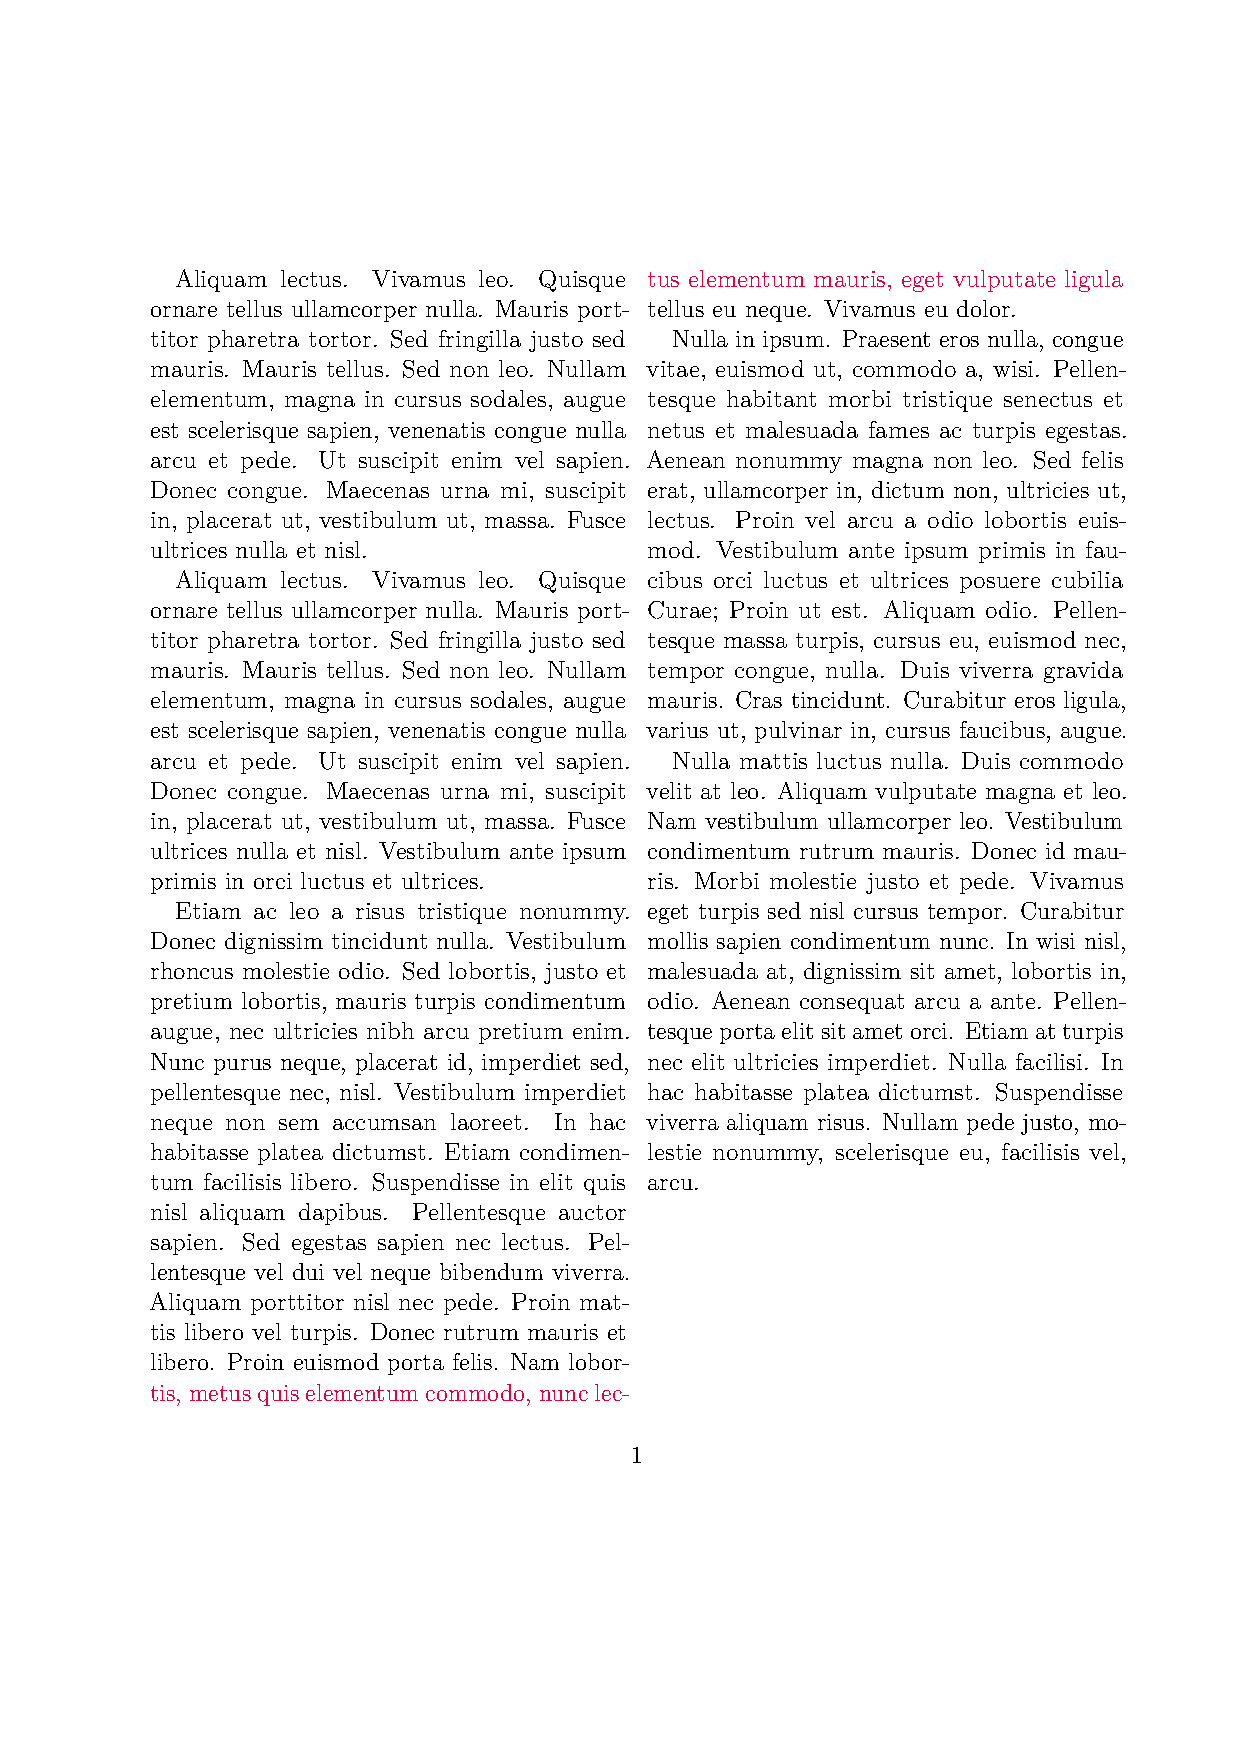
\includegraphics[height=\textheight,page=1]{examples/widow.pdf}
  \end{center}
\end{frame}

\begin{frame}
  \frametitle{Potlačený sirotek}
  \begin{center}
    \includegraphics[height=\textheight,page=2]{examples/widow.pdf}
  \end{center}
\end{frame}

\begin{frame}
  \frametitle{Porovnání různých metod k omezení parchantů}
  \begin{center}
  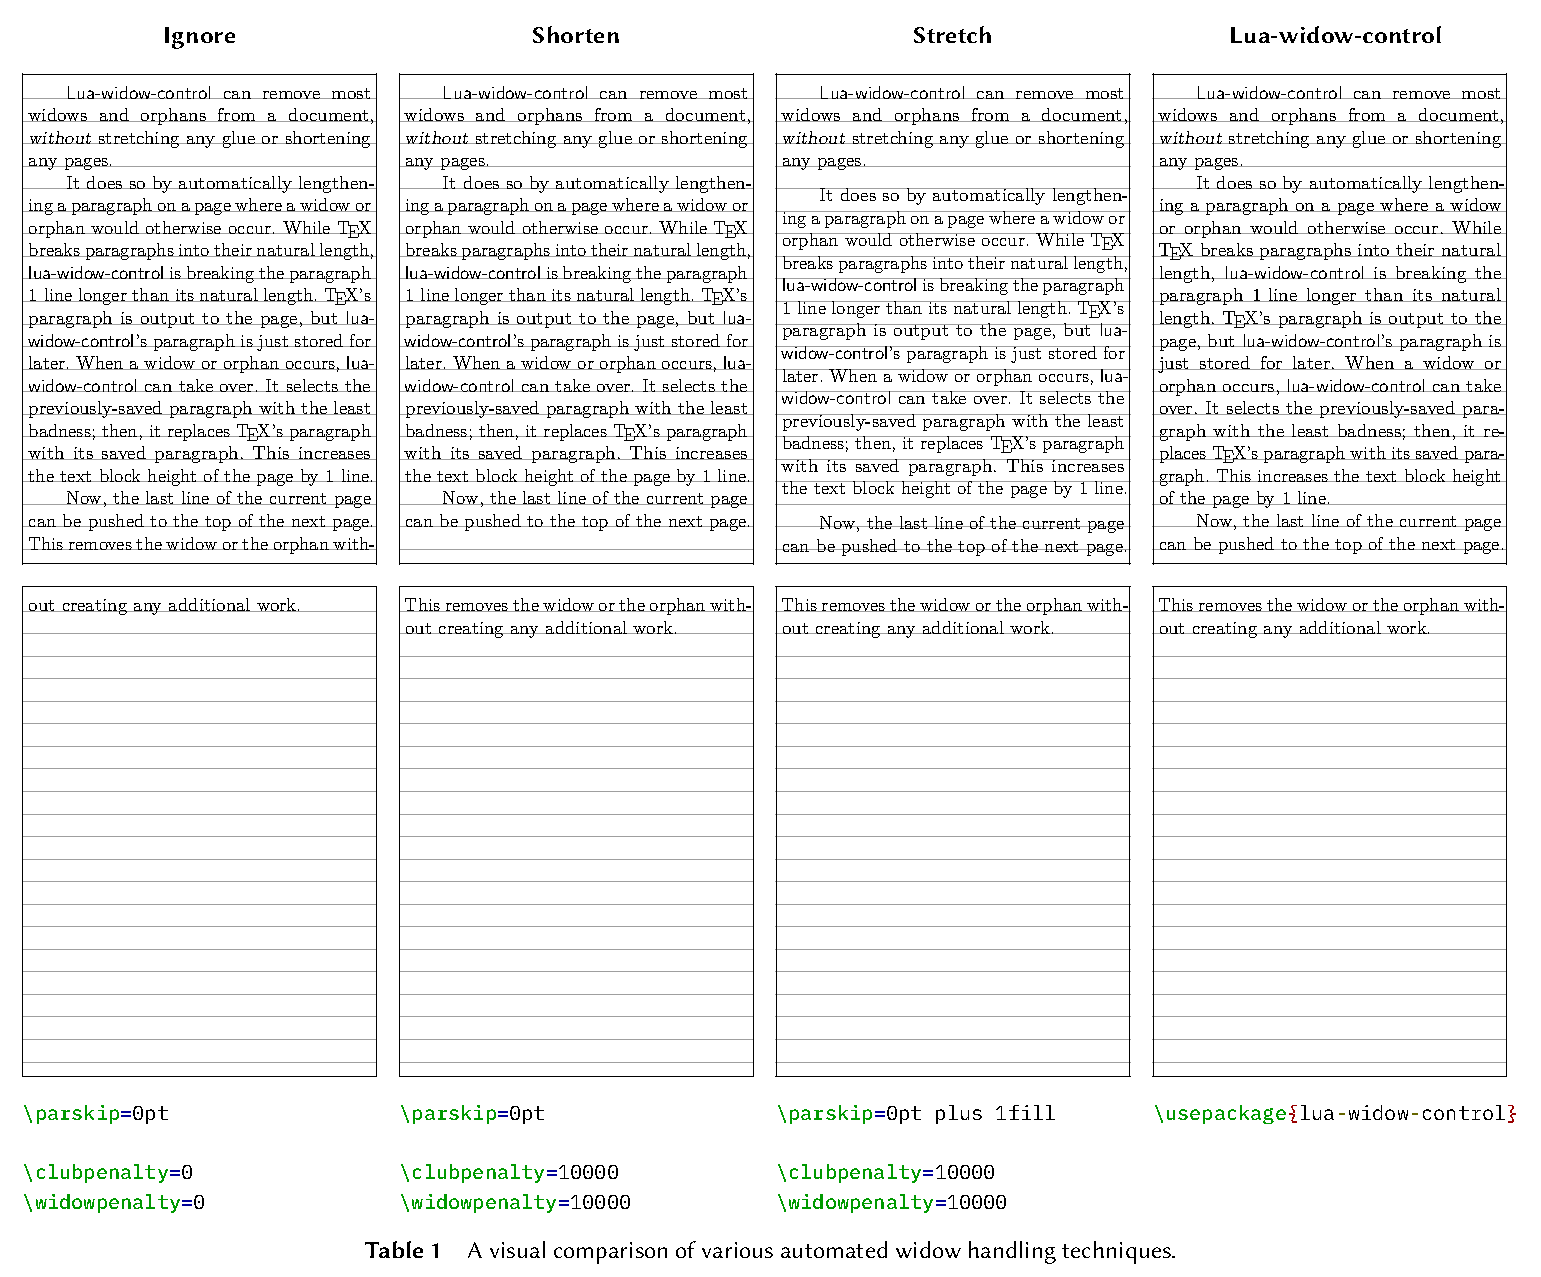
\includegraphics[height=.95\textheight]{img/lua-widow.pdf}
  \end{center}
  % \myfig[height=0.8\textheight]{img/lua-widow.pdf}{}
\end{frame}

\begin{frame}[fragile]
 \begin{verbatim}
 \lwcsetup{preset}
 \end{verbatim}
      - default - nepřidává žádné vertikální mezery, ale může vést k příliš vzdušným odstavcům
      - strict - využívá primárně vertikální mezery a nevytváří špatné odstavce,  ale odstraní jen třetinu parchantů
        - funguje špatně hlavně pro dokumenty, které obsahují jen text, beletrii apod.
      - balanced - kombinuje obě metody, odstraní 90\% parchantů
    - upozornění:
      - \verb|\clubpenalty| a \verb|\widowpenalty| nemají žádný efekt, naopak mohou způsobit vedlejší účinky
      - podpora pro více sloupcovou sazbu je omezená, balíček Multicol nefunguje
\end{frame}
  - linebreaker

 

\begin{frame}[fragile]
  \frametitle{Balíček Luavlna}
  \begin{itemize}
    \item Zamezuje rozdělení řádků:
      \begin{itemize}
        \item za jednoslovnými předložkami
        \item u akademických titulů
        \item mezi čísly a jednotkami
      \end{itemize}
  \end{itemize}
\end{frame}

\begin{frame}
  \frametitle{Ukázka užití Luavlny}
  \begin{minipage}{3in}

    \preventsingledebugon

    Text s krátkými souhláskami a samohláskami i dalšími jevy
    z nabídky možností (v textu možnými).

    Co třeba í znaky š diakritikou?

    Různé možnosti [v závorkách \textless i jiných znacích

    Podpora iniciál a titulů: M. J. Hegel, Ing. Běháková, Ph.D., Ž. Zíbrt,
    Ch. Borner.

    Podpora jednotek: 100,5 MN\cdot{}s, 100.5 kJ, 200 µA, $-1$ dag,
    12 MiB.

    Uvnitř matematiky by mělo být zpracování vypnuté: $k \in \mathbb N$.

    \preventsingledebugoff
  \end{minipage}
\end{frame}

\begin{frame}[fragile]
  \frametitle{Jak to funguje?}
  
  \begin{itemize}
    \item využíváme callback Lua\TeX u \verb|pre_linebreak_filter|
    \item zpracovává odstavce a boxy před tím, než jsou zalomené do řádků
  \end{itemize}

\end{frame}

\begin{frame}[fragile]
  \frametitle{Podporované jazyky}

\end{frame}

\begin{frame}
  \frametitle{How are hooks configured}
\end{frame}

\begin{frame}[fragile]
  \frametitle{\texttt{tex4ht.sty} package options}
  \begin{priklad}
\begin{verbatim}
$ make4ht filename.tex "mathml,mathjax"
\end{verbatim}
\end{priklad}
\end{frame}
